% section appendix
% Kota Miura (miura@embl.de)

\section{Appendices}

\subsection{App.1 Header Structure and Image Files}
\label{app1}

For TIFF format, detailed description could be found at:\\
\url{http://www.digitalpreservation.gov/formats//content/tiff_tags.shtml}

\clearpage

\subsection{App.1.5 Installing Plug-In}
\label{app1.5}
\textbf{ImageJ}

To install Plug-In, download the Plug-In file (*.class or *.jar) and put the file
in the "plugin" folder within ImageJ folder. 
ImageJ must be restarted to see the plugin in the menu. 
By default, Plug-in appears under
\ijmenu{[Plugins]}.
If you want to change the location of the plugin in the menu, one can
change the place by using \ijmenu{[Plugins > Utilities > Control Panel]}.

If you have too many Plugins, there will be significant probability of so called
"Class conflicts". Classes are the modules in ImageJ and Plugins. 
If there are two identical classes in
ImageJ, then these classes causes the conflict in the process. To avoid
this, one could have multiple ImageJ and install Plugin in each
of them for different purposes, that there will be no Plugin overloads. 

\textbf{Fiji}

Select  \ijmenu{[Plugins > Install Plugins\dots]} then choose the
plugin file (.jar or .class file). 


\clearpage
\subsection{App.1.75 List of accompanying PDF}
\label{app1.75}
\begin{itemize}
\item ImageJ\_Manual.pdf 
\subitem ImageJ Manual written by Tony Collins@Cell Imaging Core facility,
Toronto Western Research Intsitute

\item rossner\_yamada.pdf
\subitem JCB paper about manipulation of image data.

\item Time Series\_Analyzer.pdf
\subitem Manual for the Time Series Analyzer PlugIn 

\item Manual Tracking plugin.pdf
\subitem Manual Tracker PlugIn manual
\end{itemize}


\clearpage
\subsection{App.2 Measurement Options}
\label{app2}
Copied from\\
\url{http://rsb.info.nih.gov/ij/docs/guide/userguide-27.html\#toc-Subsection-27.7}

\textbf{Area}\\Area of selection in square pixels or in calibrated
square units (e.g., $mm^2$, $\mu m^{2}$, etc.) if Analyze
${\triangleright}$ Set Scale\ldots was used to spatially calibrate the
image.

\textbf{Mean Gray Value}\\Average gray value within the selection.
This is the sum of the gray values of all the pixels in the selection
divided by the number of pixels. Reported in calibrated units (e.g.,
optical density) if Analyze ${\triangleright}$ Calibrate\ldots was
used to calibrate the image. For RGB images, the mean is calculated by
converting each pixel to grayscale using the formula\\
$gray=(red+green+blue)/3$\\
or\\
$gray=0.299 red + 0.587 green + 0.114 blue$\\
if Weighted RGB Conversions is checked in Edit ${\triangleright}$
Options ${\triangleright}$ Conversions\ldots




\textbf{Standard Deviation}\\Standard deviation of the gray values
used to generate the mean gray value. Uses the Results table heading
StdDev.

\textbf{Modal Gray Value}\\Most frequently occurring gray value
within the selection. Corresponds to the highest peak in the histogram.
Uses the heading Mode.

\textbf{Min \& Max Gray Level}\\Minimum and maximum gray values
within the selection.


\textbf{Centroid}\\The center point of the selection. This is the
average of the x and y coordinates of all of the pixels in the image or
selection. Uses the X and Y headings.

\textbf{Center of Mass}\\This is the brightness-weighted average of
the x and y coordinates all pixels in the image or selection. Uses the
XM and YM headings. These coordinates are the first order spatial
moments.

\textbf{Perimeter}\\The length of the outside boundary of the
selection. Uses the heading Perim.. With IJ1.44f and
later, the perimeter of a composite selection is calculated by
decomposing it into individual selections. Note that the composite
perimeter and the sum of the individual perimeters may be different due
to use of different calculation methods.

\textbf{Bounding Rectangle}\\The smallest rectangle enclosing the
selection. Uses the headings BX, BY, Width and Height, where BX and BY
are the coordinates of the upper left corner of the rectangle.

\textbf{Fit Ellipse}\\ Fits an ellipse to the selection. Uses the
headings Major, Minor and Angle. Major and Minor are the primary and
secondary axis of the best fitting ellipse. Angle is the angle between
the primary axis and a line parallel to the X-axis of the image. The
coordinates of the center of the ellipse are displayed as X and Y if
Centroid is checked. Note that ImageJ cannot calculate the major and
minor axis lengths if Pixel Aspect Ratio in the Analyze
${\triangleright}$ Set Scale\ldots dialog is not 1.0. There are
several ways to view the fitted ellipse:
\begin{enumerate}
\item The Edit ${\triangleright}$ Selection ${\triangleright}$ Fit
Ellipse command replaces an area selection with the best fit
ellipse.

\item The DrawEllipse macro draws (destructively) the best fit ellipse and
the major and minor axis.

\item Select Ellipses from the Show: drop-down menu in the particle
analyzer (Analyze ${\triangleright}$ Analyze Particles\ldots) and it
will draw the ellipse for each particle in a separate window.
\end{enumerate}

\textbf{Shape Descriptors}\\Calculates and displays the following
shape descriptors:

\begin{itemize}
\item \textbf{Circularity}\\$4\pi\frac{Area}{\text{Perimeter}^{2}}$ with
a value of 1.0 indicating a perfect circle. As the value approaches
0.0, it indicates an increasingly elongated shape. Values may not be
valid for very small particles. Uses the heading Circ.

\item \textbf{Aspect Ratio}\\The aspect ratio of the
particle"s fitted ellipse, i.e., $\frac{[\text{Major Axis}]}{[\text{Minor
Axis}]}$. If Fit Ellipse is selected the Major and Minor axis are
displayed. Uses the heading AR.

\item \textbf{Roundness}\\$4\frac{[\text{Area}]}{\pi [\text{Major axis}]^{2}}$ or the inverse
of Aspect Ratio. Uses the heading Round.
\item \textbf{Solidity}\\$\frac{[\text{Area}]}{[\text{Convex area}]}$ ; 
Note that the 
Edit${\triangleright}$ Selection ${\triangleright}$ Convex Hull 
command makes an area selection convex.

\end{itemize}

\textbf{Feret's Diamete}r\\The longest distance
between any two points along the selection boundary, also known as
maximum caliper. Uses the heading Feret. The angle ($0-180$ degrees)
of the Feret's diameter is displayed as FeretAngle, as
well as the minimum caliper diameter (MinFeret). The length of the
object"s projection in the X (FeretX) and Y (FeretY)
direction is also displayed.

\textbf{Integrated Density}\\The sum of the values of the pixels in
the image or selection. This is equivalent to the product of Area and
Mean Gray Value. With IJ1.44c and later, Raw integrated
density (sum of pixel values) is displayed under the heading RawIntDen
when Integrated density is enabled. The Dot Blot Analysis tutorial
demonstrates how to use this option to analyze a dot blot assay.

\textbf{Median}\\The median value of the pixels in the image or
selection.

\textbf{Skewness}\\The third order moment about the mean. The
documentation for the Moment Calculator plugin explains how to
interpret spatial moments. Uses the heading Skew.

\textbf{Kurtosis}\\The fourth order moment about the mean. Uses the
heading Kurt.

\textbf{Area Fraction}\\For thresholded images is the percentage of
pixels in the image or selection that have been highlighted in red
using Image ${\triangleright}$ Adjust ${\triangleright}$
Threshold\ldots [T]. For non-thresholded images is the percentage of
non-zero pixels. Uses the heading \%Area.

\textbf{Stack Position}\\The position (slice, channel and frame) in
the stack or hyperstack of the selection. Uses the headings Slice, Ch
and Frame.

n.b.: For line selections the heading Length is created. For straight
line selections, Angle is recorded even if Fit Ellipse is unchecked.
Also, note that measurements that do not apply to certain selection
types may be listed as $NaN$, 
$Infinity$ or $-Infinity$.

The second part of the dialog controls measurement settings:

\textbf{Limit to Threshold}\\If checked, only thresholded pixels
are included in measurement calculations. Use Image ${\triangleright}$
Adjust ${\triangleright}$ Threshold\ldots [T] to set the threshold
limits. This setting affects only thresholded images (see Settings and
Preferences).

\textbf{Display Label}\\If checked, the image name and slice number
(for stacks) are recorded in the first column of the results table,
e.g., mri-stack.tif:9. For renamed selections (Edit ${\triangleright}$
Selection ${\triangleright}$ Properties\ldots [y]) or selections
measured via ROI Manager"s measure command (see ROI
Manager\ldots), the selection label is appended, e.g.,
blobs.gif:0339-0163 or blobs.gif:mySelection.


\textbf{Invert Y Coordinates}\\If checked, the XY origin is assumed
to be the lower left corner of the image window instead of the upper
left corner (see also Image ${\triangleright}$ Properties\ldots [P]).

\textbf{Scientific Notation}\\If checked, measurements are
displayed in scientific notation, e.g., 1.48E2.

\textbf{Redirect To}\\The image selected from this pop-up menu will
be used as the target for statistical calculations done by Analyze
${\triangleright}$ Measure\ldots [m] and Analyze ${\triangleright}$
Analyze Particles\ldots commands. This feature allows you to outline a
structure on one image and measure the intensity of the corresponding
region in another image.

\textbf{Decimal Places}\\This is the number of digits to the right
of the decimal point in real numbers displayed in the Results table and
in Histogram windows.


\clearpage


\subsection{App.3 Edge Detection Principle }
\label{app3}
Quote from MBL manual: 

\begin{quote}
One way to find boundaries of objects is to detect discontinuities in
intensity values at the edge of a region. These discontinuities can
be found by calculating the first and/or second order derivatives of an
image. The first derivative of choice in image processing is the
gradient, defined as the vector:

\[
grad\, f=[G_{x}G_{y}]
\] 

where 
$G_{x}=df/dx$ 
 and
$G_{y}=df/dy$ 
 are the partial derivatives in the horizontal and
vertical directions of the image. The magnitude of this vector is
\[
\left |  grad\, f\right |=(G_{x}^{2}+G_{y}^{2})^{1/2}
\]

The gradient vector points in the direction of steepest ascent. The
angle of steepest ascent is given by:
\[
a(x,y)=tan^{-1}(G_{x}/G_{y})
\]

We can estimate the derivatives $G_{x}$ and $G_{y}$ digitally by linearly
filtering the image with the following 3 by 3 kernels: 

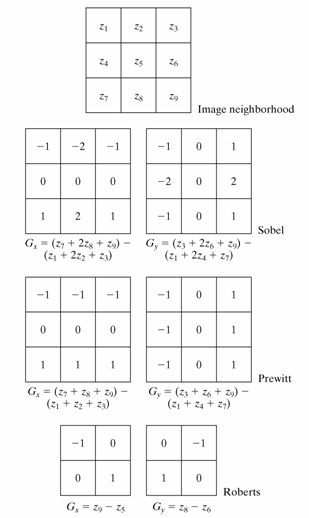
\includegraphics[width=6.653cm,height=8.221cm]{fig/CMCIBasicCourse201102-img153.png}

The Prewitt and Sobel operators are among the most used in practice for
computing digital gradients. The Prewitt masks are simpler to
implement than the Sobel masks, but the latter have slightly superior
noise-suppression characteristics.
\end{quote}

\clearpage

\subsection{App.4 Particle Tracker manual}
\label{app4}

Tutorial from : \url{http://weeman.inf.ethz.ch/particletracker/tutorial.html}

PDF inserted from next page. 

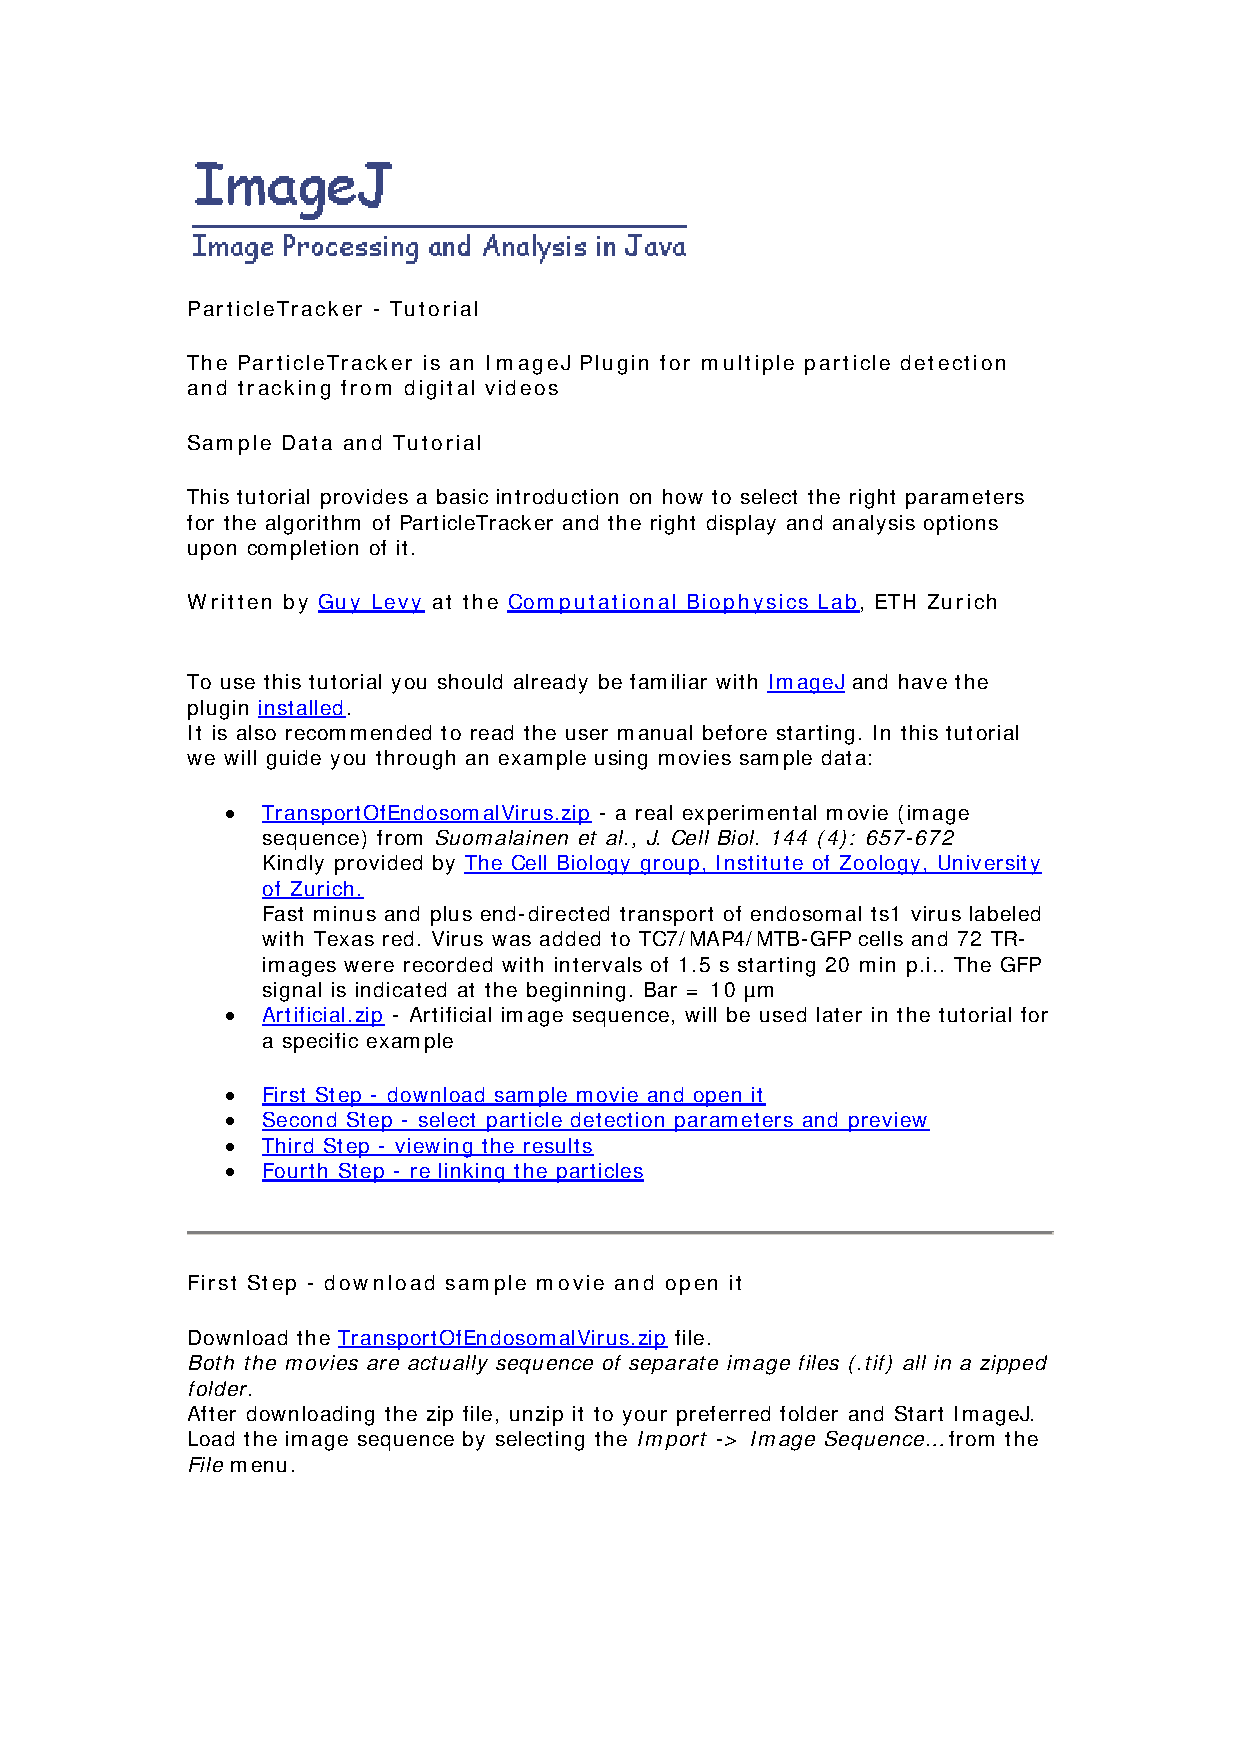
\includepdf[pages=-]{pdf/ParticleTrackertutorial.pdf}

\clearpage
\subsection{App.5 Particle Analysis}
\label{app5}
Copied from ImageJ website:

"Particle Analysis" counts and measures
objects in binary or thresholded images. It works by scanning the image
or selection until it finds the edge of an object. It then outlines the
object using the wand tool, measures it using the Measure command,
fills it to make it invisible, then resumes scanning until it reaches
the end of the image or selection. Press the esc key to abort this
process. Use Image/Adjust/Threshold to threshold an image.



Use the dialog box to configure the particle analyzer. Particles outside
the range specified in the Size field are ignored. Enter a single value
in Size and particles smaller than that value are ignored. Particles
with circularity values outside the range specified in the Circularity
field are also ignored. The formula for circularity is
4pi(area/perimeter\^{}2). A value of 1.0 indicates a perfect circle.
Note that the Circularity field was added in ImageJ 1.35e.

Select Outlines from the "Show:" pop-up menu
and ImageJ will open a window containing numbered outlines of the
measured particles. Select Masks to display filled outlines of the
measured particles or Ellipses to display the best fit ellipse of each
measured particles.

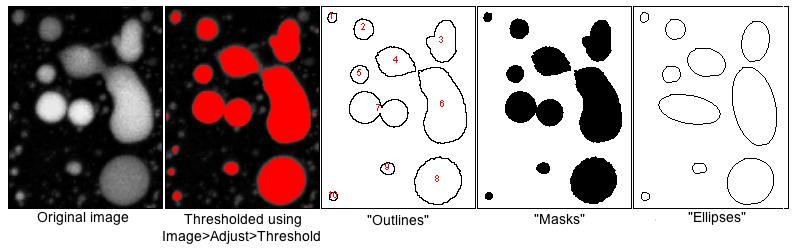
\includegraphics[width=12cm]{fig/CMCIBasicCourse201102-img169.jpg}

Check Display results to have the measurements for each particle
displayed in the "Results" window. Check
Clear Results to erase any previous measurement results. Check
Summarize to display, in a separate window, the particle count, total
particle area, average particle size, and area fraction. Check Exclude
on Edges to ignore particles touching the edge of the image or
selection.

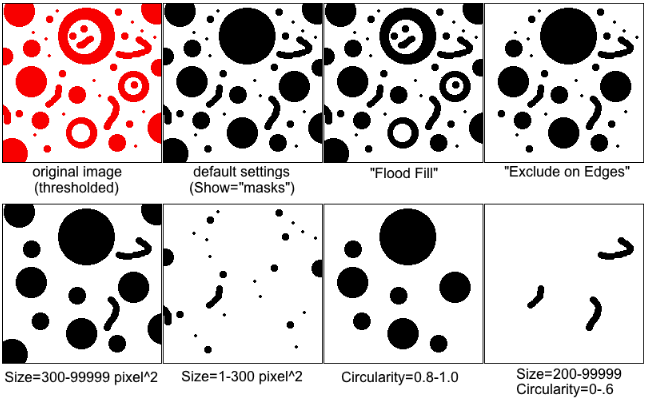
\includegraphics[width=12cm]{fig/CMCIBasicCourse201102-img170.png}

Check Flood Fill and ImageJ will define the extent of each particle by
flood filling instead of by tracing the edge of the particle using the
equivalent of the wand tool. Use this option to exclude interior holes
and to measure particles enclosed by other particles. The following
example image contains particles with holes and particles inside of
other particles.


\clearpage

\subsection{App.6 Image Processing and Analysis: software, scripting language}
\label{app6}

ImageJ is not only the tool for scientific image processing and
analysis. I list some other software and tools used by EMBL researchers
here and add some description about each of them. For more details, please refer to an article by \citet{WalterNATM2010}.

\textbf{MatLab (Mathworks), \$}

With Matlab, you could access images as numerical matrix to do
processing and analysis of images. Programming is possible with Matlab
scripting language. Scripts could be kept as files and execute them
directly from the Matlab command line. These files are called
"m-files". Many imaging related
tools are publicly available via Internet download. Scripts could be
exported as execution files, and could be distributed without Matlab
itself, as these stand-alone execution files only require freely
available Matlab library. A free alternative is Octave. I have never
tried this yet, but this freeware is under extensive development and
worth for some trial. 



\textbf{Imaris (Bitplane), \$}



Imaris is also a commercial software, especially powerful in interactive
3D visualization. 3D time course (sometimes called
"4D") with multiple channels (then
this would be called 5D) could also be visualized and interactively
adjusted with their appearance. Some analysis packages are optionally
available. I sometimes use optional package "Imaris
Track" for tracking spotty signals. Algorithm for
linking particles is excellent (uses graph-theory based algorithm
developed in Danuser lab). In EMBL, you could try using this software
by so called "floating license",
which enables you to use the software from any computer within EMBL
domain. The number of simultaneous usage is limited to three (as of
June 2010). Another module that gives additional power to Imaris is
"Imaris XT", which enables
accessing Imaris objects from Matlab, Java or ImageJ. I have some
example Java codes, so if you are interested I could give you as an
example. Imaris is pretty expensive, and apparent disadvantage. 



\textbf{Python, Free}

Python is not a software package, but is a scripting language. There are
many other scripting languages like Ruby, but the merit of Python is
that there are numerous libraries for image processing and analysis. In
terms of scripting, accessibility is similar or more powerful than
Matlab, since its bridging capability to many computer languages such
as C, C\textsuperscript{++} and Java. Considering that the trend of
image processing and analysis is getting more and more towards
cross-language library usage, Python is a good choice to learn for
high-end processing and analysis.

\textbf{Cell Profiler, Free}

This free software is a bit less with available functions compared to
ImageJ, but is easier and robust in constructing pipelines for image
processing and analysis. One could interactively construct pipeline and
do high-throughput processing and analysis for many data. 



\clearpage
\subsection{App.7 Macro for Generating Striped images}
\label{app7}

Below is an ImageJ macro code for generating stripes to do some
experiments on FFT. You could copy \& paste this in a new macro window
and install to generate stripes with various frequencies and orientation.  

\lstinputlisting[numbers=none]{MacrostripeGenerator.ijm}
\clearpage

\subsection{App.8 Deconvolution Exercise}
\label{app4}

Exercise starts from next page. 

In this exercise, following plugins are used. If you do not have them in your
ImageJ or Fiji, download them and install. Deconvolution lab cannot be installed
by \ijmenu{[Plugins > Install]}. Unpack the downloaded zip folder and place all
the contents under plugins directory.

\begin{enumerate}
	\item PSFgenerator \url{http://bigwww.epfl.ch/algorithms/psfgenerator/}
	\item DeconvolutionLab \url{http://bigwww.epfl.ch/algorithms/deconvolution/}
\end{enumerate}

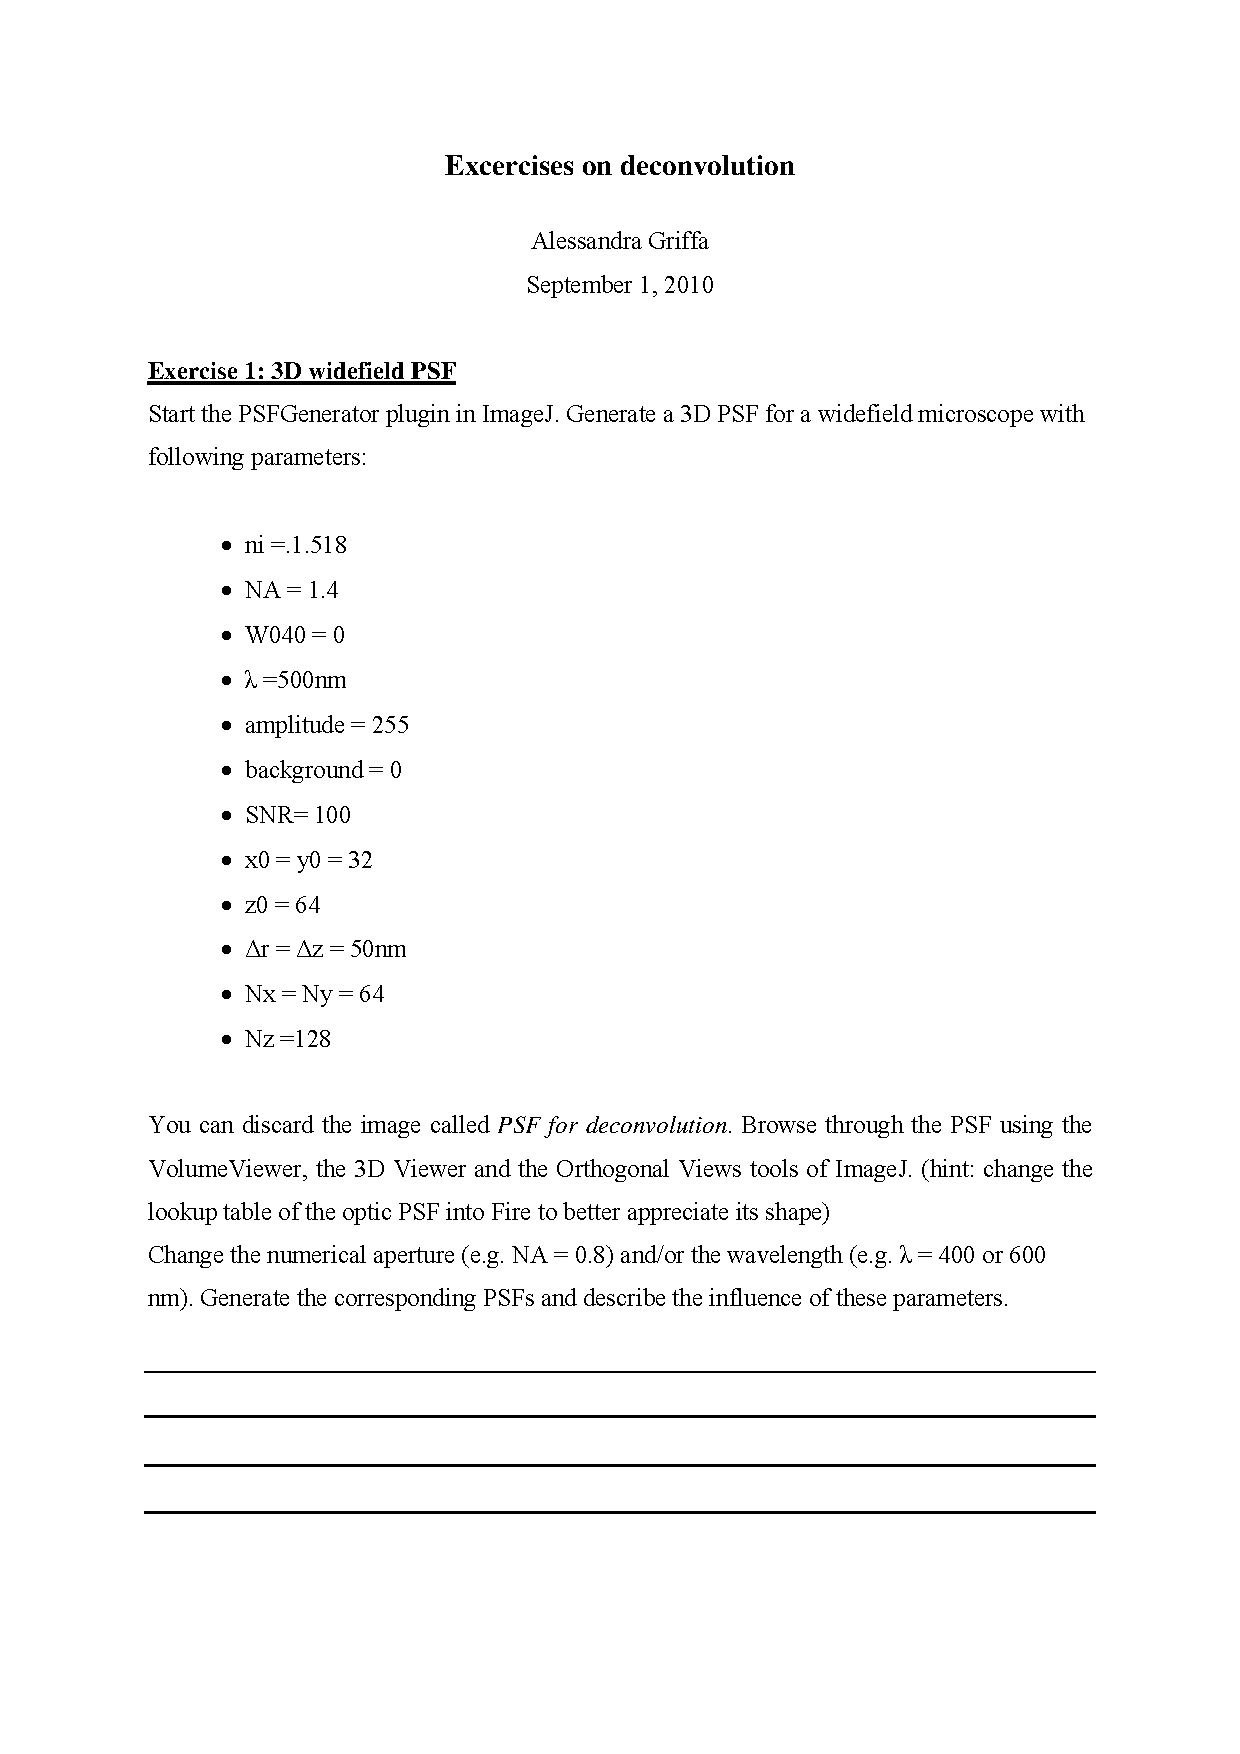
\includepdf[pages=-]{pdf/decon_exercisesIJ.pdf}

\clearpage
